% Figure 2 — live-ledger interval coverage by horizon (standalone, auto-cropped).
% Compile: pdflatex figure2_coverage.tex  ->  figure2_coverage.pdf
\documentclass[border=2pt]{standalone}
\usepackage{mathptmx}
\usepackage{amsmath,amssymb}
\usepackage{tikz}
\usepackage{pgfplots}
\pgfplotsset{compat=1.17}
\begin{document}
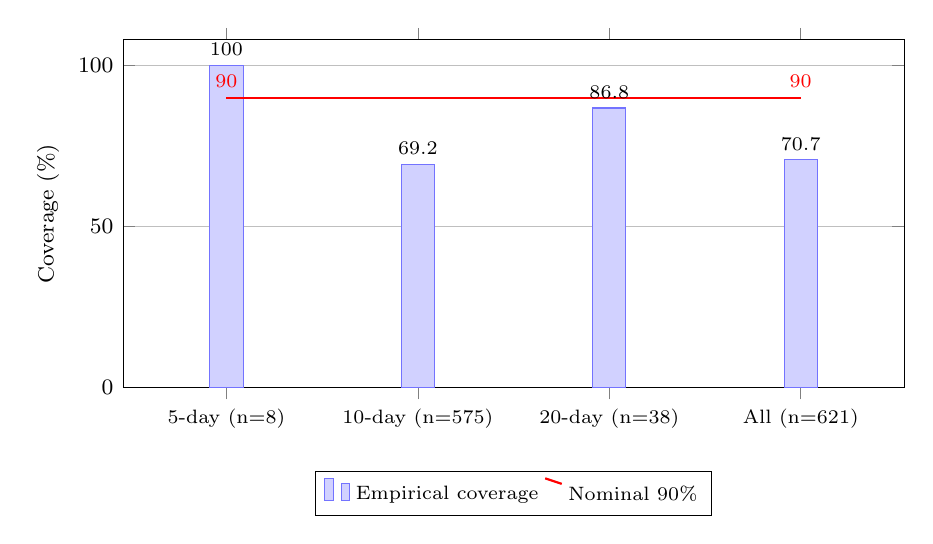
\begin{tikzpicture}
\begin{axis}[
  width=11.5cm, height=6.0cm, font=\footnotesize,
  ybar, bar width=12pt,
  symbolic x coords={5-day (n=8),10-day (n=575),20-day (n=38),All (n=621)},
  xtick=data, x tick label style={font=\scriptsize},
  ymin=0, ymax=108, ylabel={Coverage (\%)},
  enlarge x limits=0.18, ymajorgrids,
  legend style={at={(0.5,-0.24)},anchor=north,legend columns=2,font=\scriptsize},
  nodes near coords, every node near coord/.append style={font=\scriptsize}
]
\addplot[fill=blue!18,draw=blue!55] coordinates {(5-day (n=8),100.0)(10-day (n=575),69.2)(20-day (n=38),86.8)(All (n=621),70.7)};
\addplot[sharp plot,thick,red,mark=none,update limits=false] coordinates {(5-day (n=8),90)(All (n=621),90)};
\legend{Empirical coverage, Nominal 90\%}
\end{axis}
\end{tikzpicture}
\end{document}
